\documentclass[12pt,german]{article}
\usepackage{listings}
%\usepackage[utf8]{inputenc}
\usepackage{inputenc}
\usepackage{graphicx}
\usepackage{float}
\usepackage{array}
\usepackage{pdfpages}

\lstset{
extendedchars=\true,
language=JAVA,
%inputencoding=utf8,
%basicstyle=\ttfamily,
%basicstyle=\ttfamily\fontsize{8}{8},
%commentstyle=\ttfamily\fontsize{8}{8},
basicstyle=\tiny;
columns=fullflexible,
%xleftmargin=5pt,
frame=single,
breaklines=true,
postbreak=\mbox{{$\hookrightarrow$}\space},
}
\renewcommand{\thesubsubsection}{\alph{subsubsection} )}
%\renewcommand{\thesubsubsection}{\thesubsection.\alph{subsubsection} )}

\setcounter{section}{1}

\begin{document}

\title{Übungsaufgaben II, SBV1 }
\author{Lukas Fiel, Lisa Panholzerl}
\maketitle


\newpage
\section{Übungsaufgaben II}
\subsection{Resampling und Interpolation}
\subsubsection{Implementierung Resampling}
Die Implementierung des Resampling Filters wurde in diesem Abschnitt anhand der Nearest Neighbour Interpolation umgesetzt. Bevor der Filter ausgeführt wird, wird zuerst der Skalierungsfaktor bei dem Benutzer abgefragt. Gibt der Benutzer einen positiven Wert ein, der über dem Default-Wert von 2.0 liegt, wird das Bild vergrößert. Gibt er einen negativen Wert ein wird das Eingangsbild verkleinert.

In dieser Implementierung wird die Umrechnung der Koordinaten anhand der Variante B umgesetzt. Dies bedeutet, dass der Skalierungsfaktor bereits vor der Neuberechnung der Koordinaten angepasst wird, in dem von diesem 1 subtrahiert wird. Das heißt, die neue Koordinate vom skalierten Bild B wird mit der Koordinate aus dem Originalbild A um den adaptierten Skalierungsfaktor s' multipliziert. Dies hat zur Folge, dass sich die Indizes in der Mitte zentrieren. Der Anfang bzw. das Ende des Bild Arrays bleibt hierbei aber weiterhin unterrepräsentiert.\\

\lstinputlisting[frame=single,language=JAVA,breaklines=true]{../../Resample_.java}

\subsubsection{Implementierung Bi-Lineare Interpolation}
Die Implementierung des Resamplings Filters wurde in diesem Abschnitt anhand der Bilinearen Interpolation umgesetzt. Bevor der Filter ausgeführt wird, wird zuerst der Skalierungsfaktor bei dem Benutzer abgefragt. Gibt der Benutzer einen positiven Wert ein, der über 1.0 liegt, wird das Bild vergrößert. Gibt er einen darunterliegenden Wert ein wird das Eingangsbild verkleinert.

Danach wird die neue Höhe und Breite des Eingangsbildes anhand des Skalierungsfaktor berechnet. Zusätzlich wird der Skalierungsfaktor für die x und y Koordinaten separat berechnet und gespeichert. Anschließend wird anhand einer for-Schleife über alle Pixel des neu angelegten Arrays des skalierten Bildes iteriert. 

TODO: Das mit den vier Pixel suchen beschreiben und weniger details.

Neben der neuen Koordinate wird der Pixelwert anhand der Methode GetBilinearInterpolatedValue() berechnet. Hierbei werden für die Berechnung des Wertes zuerst Teile der Kalkulation in Variablen gespeichert. In diesem Fall das deltaX, deltaY, sowie die Offset-Werte. Anschließend werden noch die Offset-Werte wieder auf ihren ursprünglichen Wert gesetzt, wenn die Iteration über alle Pixel an den Bildrändern ankommt. 


Um den gewichtet Mittelwert für diesen Pixel zu erhalten, werden zuerst die skalaren Werte der 4 benachbarten Pixel in Variablen gespeichert. Anhand der Kalkulationsfragmente, den benachbarten skalaren Werte kann nun der gewichtete Mittelwert berechnet werden. Anschließend wird dieser Wert an die Methode retourniert und im skalierten Bild an der aktuellen Koordinate eingefügt.

TODO: Testbild einfügen

TODO: Differenzbild einfügen (Image J Funktionalität)

TODO: Unterschied in skalare Werte, woher? \\

\lstinputlisting[frame=single,language=JAVA,breaklines=true]{../../ResampleBilineareInterpolation_.java}


\subsubsection{Implementierung Checker-Board}
TODO: Charakterisierung der beiden Interpolationsstrategien auf Laufzeit und erzielbare Qualität

 NN = einfacherer Algorythmus --> kürzere Laufzeit
BIP = kompolexerer Algorythmus --> längerer Laufzeit

NN --> kantigeres Ergebnis, da keine Neuberechnung des skalaren Wert stattfindet, sondern eine neue Zuweisung
BIP --> weicheres Ergebnis, da der skalare Wert aus den 4 Nachbarn und dem Delta berechnet wird


\subsection{Klassifizierung mittels Kompression}
\subsubsection{Klassifizierung von Texten}

\textbf{Idee}

Aus Texten in 8 verschiedenen Sprachen soll mittels Kompression eine Klassifizierung stattfinden. Dazu wurden folgende Datensätze als \" *.txt \" Datein vorbereitet:

\begin{itemize}
	\item Abstract einer wissenschaftlichen Arbeit. Diese hatte den Vorteil dass es eine deutsche und englische Übersetzung gab. Alle weiteren Sprachen wurden aus der englischen Version mittels \textit{google translate} generiert.
	\item Wörterbuch mit 10000 deutschen Wörtern. Dieser Datensatz wurde mittels \textit{google translate} in alle anderen Sprachen übersetzt.
	\item Die erste Seite der Datenschutzrichtlinien von Facebook. Da die Datenschutzrichtlinien in sämtlichen Sprachen abrufbar sind, konnte für alle Sprachen ein passender Datensatz gefunden werden.
	\item Die erste Seite der Datenschutzrichtlinien von Google. Auch hier waren Daten in allen Sprachen verfügbar.
	\item Ein Witz der aus dem deutschen mittels \textit{google translate} in alle andern Sprachen übersetzt wurde.
\end{itemize}

Da nach einer Übersetzung die Texte in verschiedenen Sprachen ungleich viele Buchstaben beinhalten ist auch die Dateigröße unterschiedlich. Dies könnte eventuell rechnerisch berücksichtigt werden. Viel einfacher aber ist es, die letzten Buchstaben jedes langen Textes zu ignorieren und so eine einheitliche Länge des Textes zu gewährleisten. Dies wurde mittels eines shell-Skripts erreicht, welches nur die ersten $n$ Bytes eines Files speichert. So konnte für jeden Text eine Datei erzeugt werden die in allen Sprachen den selben Speicherbedarf hat. Der Verlust der letzten Byte ist bei einer Klassifizierung unwesentlich. 

\lstinputlisting[frame=single,language=MATLAB,breaklines=true]{../cutData.sh}

Nach einer solchen Normierung der Texte können diese miteinander verglichen werden. Dazu wurde ein Programm in \textit{Octave} geschrieben (siehe Listing \ref{fig: calculateMatrixOctaveCode}  , welches die Texte der einzelnen Datensätze miteinander vergleicht und in einer Matrix darstellt. Eine qualitativ hochwertige Aussage ob die Ergebisse statistische Aussagekraft haben, kann mit $5$ Datensätzen nicht getroffen werden. Es ist aber sicherlich ein Trend erkennbar.


\begin{figure}[H]
	\centering
	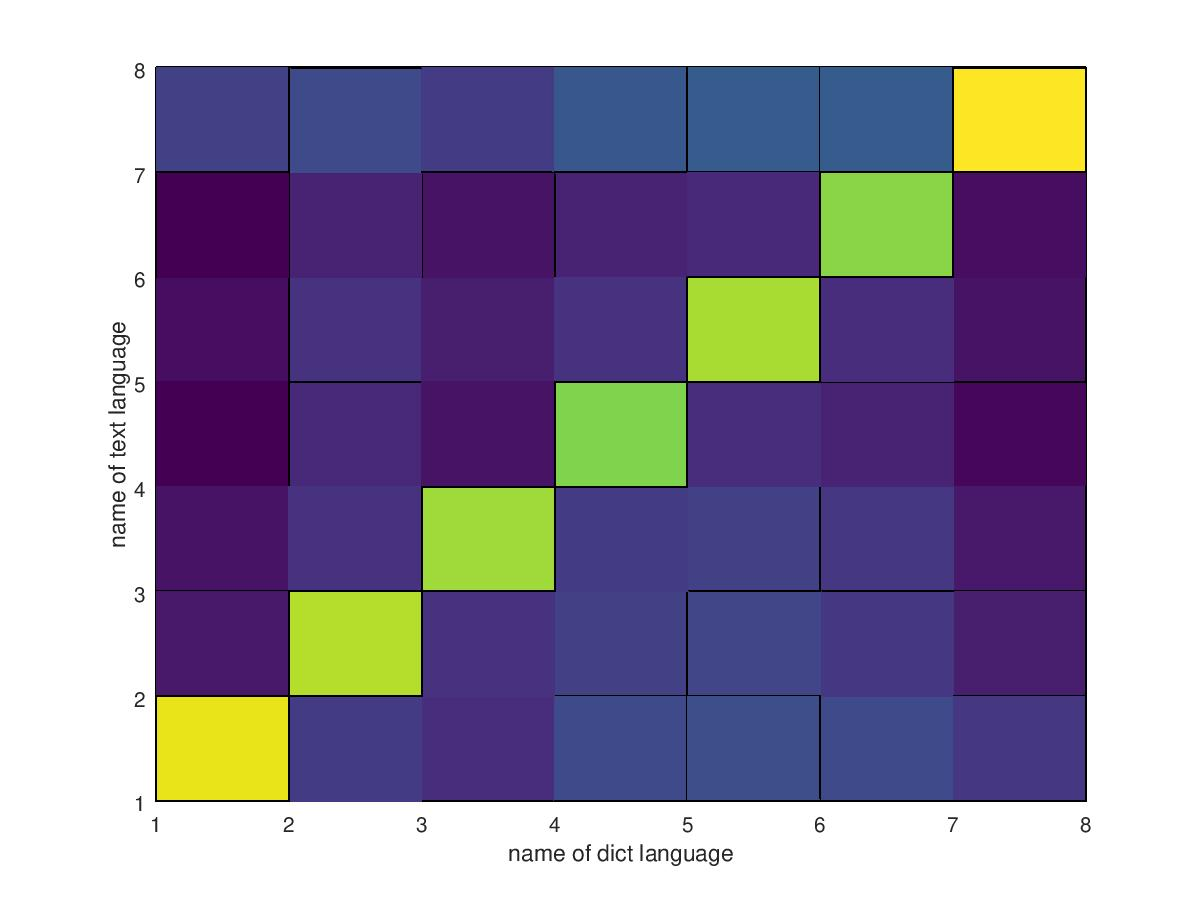
\includegraphics[width=12cm]{images/resultZipData.jpg}
	\caption{zipDataMatrix}
	\label{fig: zipDataMatrix}
\end{figure}

\newpage
\lstinputlisting[frame=single,language=MATLAB,breaklines=true,caption = Octave Script zur Darstellung der einzelnen Kompressionsraten.]{../calculateZipMatrix.m}
\label{fig: calculateMatrixOctaveCode}


\subsubsection{OPTIONAL – nur für Interessierte/Experten}


\subsection{Kompression und Code-Transformation}
\subsubsection{Lempel-Ziv Kompression einer Sequenz}
Figure \ref{fig: manualLemperZivPdf} zeigt die händische Berechnung der Lemper Ziv Kompression. Beim Übertragen ins Protokoll wurde allerdings ein Fehler entdeckt, der in Tabelle \ref{tab:Level Ziv Kompression} korrigiert wurde.



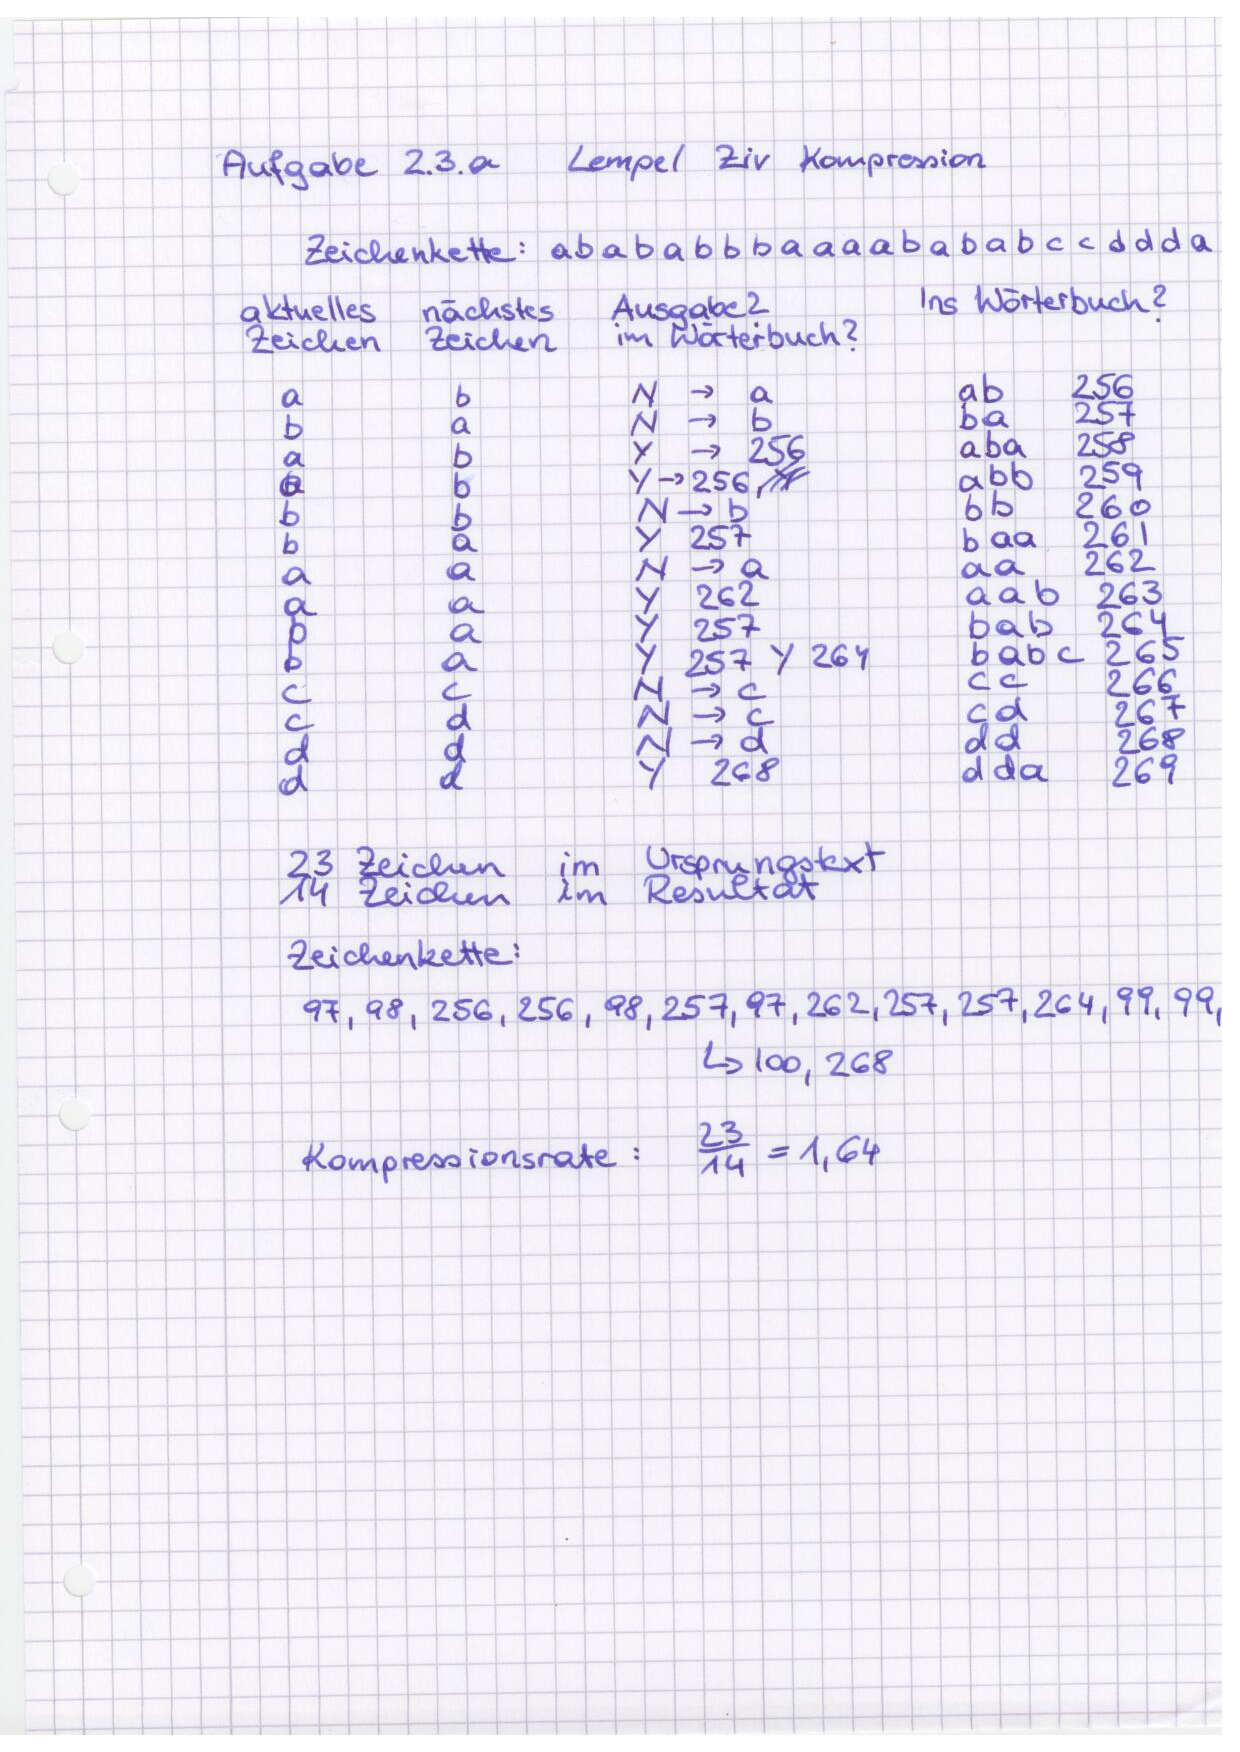
\includepdf[scale=0.4]{images/lemperZiv.pdf}
\label{fig: manualLemperZivPdf}


\begin{table}[H]
  \centering
  \begin{tabular}{c | c | c | c | c |}
    \hline
   	aktuelles  & nächstes  & Ausgabe  & ins & Speicher \\
   	 Zeichen &  Zeichen &  (im Wörterbuch?) & Wörterbuch! &  \\
	a & b & N $ \rightarrow $ a & ab & 256 \\
	b & a & N $ \rightarrow $ b & ba & 257 \\
	a & b & Y $ \rightarrow $ 256 & aba & 258 \\
	a & b & Y $ \rightarrow $ 256 & abb & 259 \\
	b & b & N $ \rightarrow $ b & bb & 260 \\
	b & a & Y $ \rightarrow $ 257 & baa & 261 \\
	a & a & N $ \rightarrow $ a & aa & 262 \\
	a & a & Y $ \rightarrow $ 256 & aab & 263 \\
	b & a & Y $ \rightarrow $ 257 & bab & 264 \\
	b & a & Y (257), Y $ \rightarrow $ 264 & babc & 265 \\
	c & c & N $ \rightarrow $ c & cc & 266 \\
	c & d & N $ \rightarrow $ c & cd & 267 \\
	d & d & N $ \rightarrow $ d & dd & 268 \\
	d & d & Y $ \rightarrow $ 268 & dda & 269 \\
	a &   & N $ \rightarrow $ a &     &   \\ 
   	
  \end{tabular}
  \caption{Level Ziv Kompression}
  \label{tab:Level Ziv Kompression}
\end{table}

In der korrigierten Version ergibt die resultierende Zeichenkette: 

\begin{table}[H]
  \centering
  \begin{tabular}{| c | c | c | c | c | c | c | c | c | c | c | c | c | c | c |}
    \hline
    97 & 98& 256 & 256 & 98 & 257 & 97 & 262 & 257 & 264 & 99 & 99 & 100 & 268 & 269 \\
    \hline
  \end{tabular}
\end{table}


\begin{equation}[H]
 Kompressionsrate C = \frac{23}{15} = 1.5334	
\end{equation}


\subsubsection{Huffmann Coding}

Die nächste Seite zeigt die händische Berechnung des Huffmann Baums zum gegebenen Beispiel. Die mittlere Codewortlänge lieght dabei bei $1.869 bit $. \\

Weiters kann man auf der darauffolgenden Seite die manuelle Berechnung von 6 Testfällen finden. Es kann gesagt werden, dass die Huffmann Kompression sehr gut geeignet wäre um Daten zu komprimieren, die sehr oft gleich sind. Dabei spielt homogenität keine Rolle, sondern rein die Häufigkeit des Auftretens der Sonderfälle. An diser Stelle sei erwähbt, dass die Information über solche Sonderfälle nicht verlohren geht, sondern einfach mehr Speicher benötigt (verlusstfreies Komprimieren)

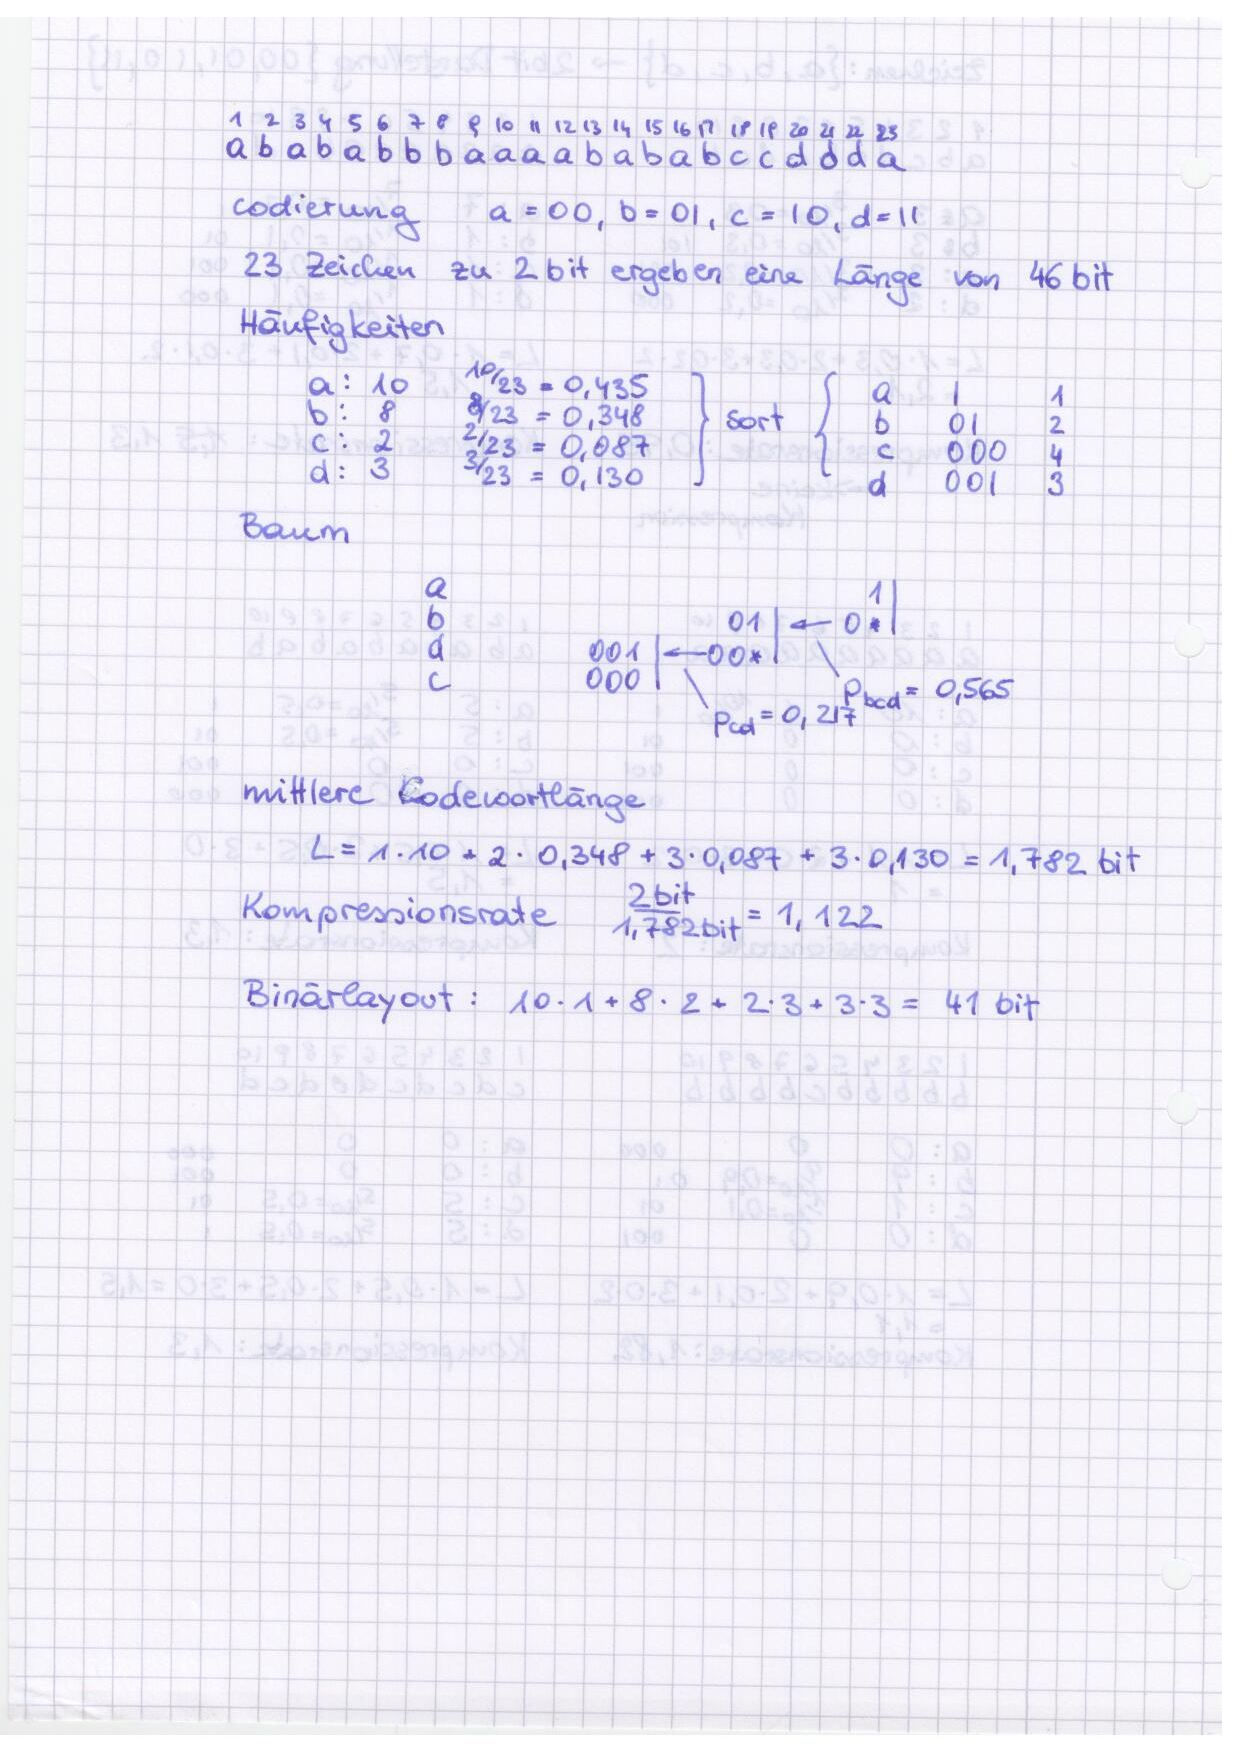
\includepdf{images/huffmannBerechnung.pdf}
\label{fig:huffmannCalculation}

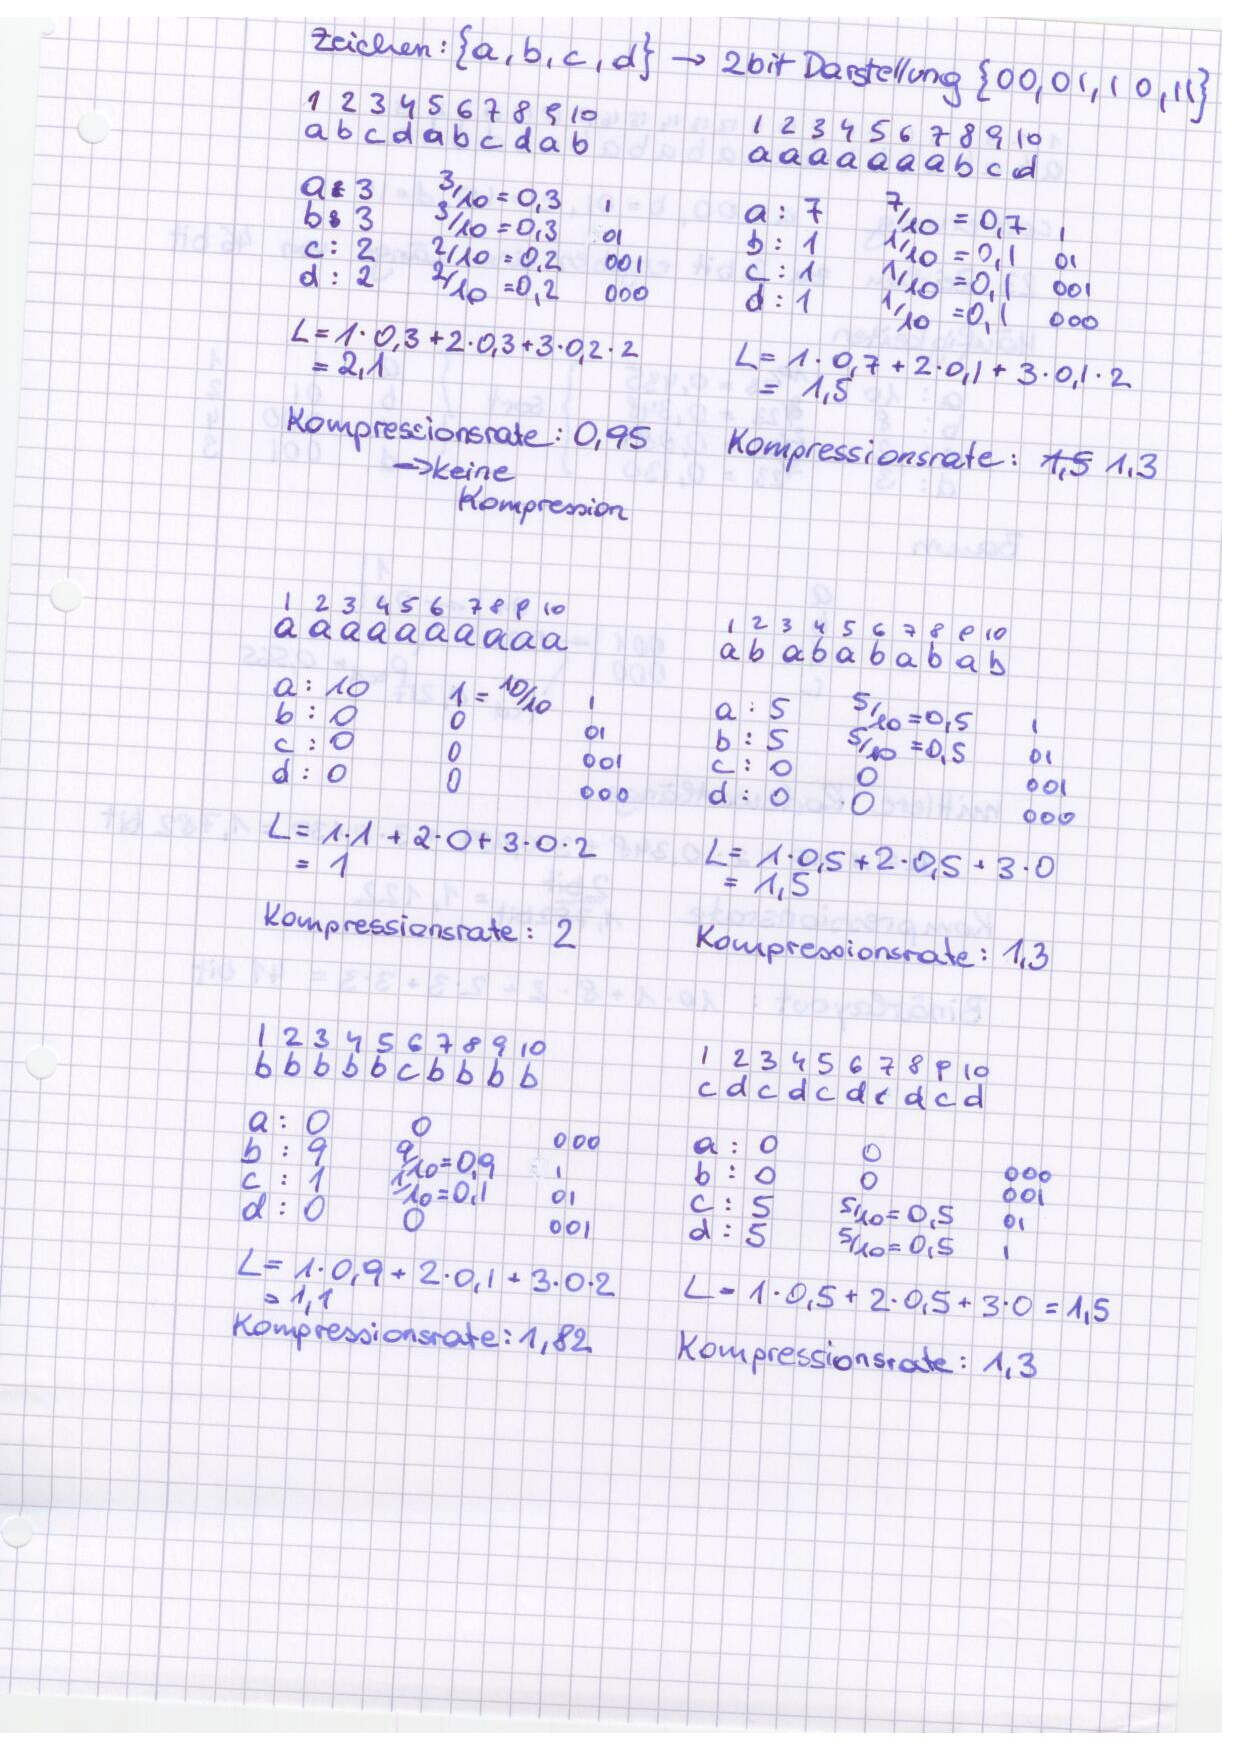
\includepdf{images/huffmannTestfaelle.pdf}
\label{fig:huffmannCalculation}


\subsubsection{Komprimierung einer Sequenz mittels Runlength Coding}
\textit{Berechnung der Kompressionsrate} 

Die nachfolgende Sequenz soll anhand von Runlength Coding händisch komprimiert und die Kompressionsrate ausgegeben werden:

010101111100000111100010101111 (30 Stellen, n=2 Symbole:0,1) \\

Die Sequenz wird von links nach rechts codiert, und anstatt der eigentlichen Zeichen die Häufigkeit dieser ausgegeben. Nach der händischen Komprimierung weist die Frequenz folgende Lauflänge auf:

11111554311114 (14 Stellen)\\


Daraus ergibt sich folgende Kompressionsrate:

30/14 = \textbf{ 2,14}\\

\textit{Erweiterung der Symbolmenge}\\
Die Komprimierung von Sequenzen anhand der RLC ist am effektivsten, je homogener der Informationsgehalt ist. Das bedeutet, das bei vielen unterschiedlichen Zeichen die Komprimierungsmethode nicht mehr sinnvoll angewandt werden kann. Bei sehr kurzen Sequenzen kann es sogar zu einer Erhöhung der Zeichenanzahl in dieser kommen.\\

Wird nun die Anzahl der Symbole erhöht, muss beachtet werden, dass zusätzlich zu der Häufigkeit des Zeichens noch ein Trennsymbol, eine ID bzw. das Zeichen selbst mitgegeben werden muss. Dies wird anhand eines selbst gewählten Beispiels demonstriert.\\

Folgende Sequenz wird anhand von RLC komprimiert:

AABBBBBBBBCCCCCCCDEEEEEEEFFGHIIJJJKLMNNN\\ (40 Stellen, n=13 Symbole:A,B,C,D,E,F,G,H,I,J,K,L,M,N)\\

Die komprimierte Sequenz lautet:

A2B8C7D1E7F2H1I2J3K1L1M1N3 (26 Stellen)\\

Daraus ergibt sich folgende Kompressionsrate:

40/26=\textbf{1,54}\\

Wird eine sehr kurze Sequenz mit einer hohen Anzahl an Symbolen komprimiert, kann es aufgrund des hohen Informationsgehalts dazu kommen, dass die codierte Sequenz länger ist, als die Originale.\\


Folgende Sequenz wird anhand von RLC komprimiert:

ABBCDEEFFFGHIIJJJKLLLMNOPQRSTU\\ (30 Stellen, n=21 Symbole:A,B,C,D,E,F,G,H,I,J,K,L,M,N,O,P,Q,R,S,T,U)\\

Die komprimierte Sequenz lautet:

A1B2C1D1E2F3G1H1I2J3K1L3M1N1O1P1Q1R1S1T1U1 (42 Stellen)\\

Daraus ergibt sich folgende Kompressionsrate:

30/42=\textbf{0,71}\\

\subsubsection{Entropieberechnung}
Folgende Sequenz zur Entropieberechnung ist gegeben:

111122661112233334564511211111 (n=6 Symbole: 1,2,3,4,5,6)\\

\textit{Minimale und Maximale Entropie}\\
Bei welcher 10-stelligen Sequenz ist die Entropie maximal bzw. bei welcher 10-stelligen Sequenz ist die Entropie minimal? 

\textit{Auswirkung auf Kompressionsrate}\\
Welche Auswirkungen hat die Entropie in Bezug auf die erzielbare Kompression?
Ist für die erzielbare Kompressionsrate dabei immer lediglich die Auftrittswahrscheinlichkeit entscheidend?


\end{document}
